Per creare una presentazione è necessario prima selezionare il progetto dalla lista dei progetti disponibili. Una volta selezionato il progetto apparirà al centro dello schermo il titolo del progetto scelto, un'immagine di anteprima della prima slide del progetto e sotto a questa un menù. Selezionando dal menù la voce \textbf{Edit} si accederà alla pagina relativa alla creazione della presentazione, con le relative funzioni.

\begin{figure}[H] 
	\centering 
	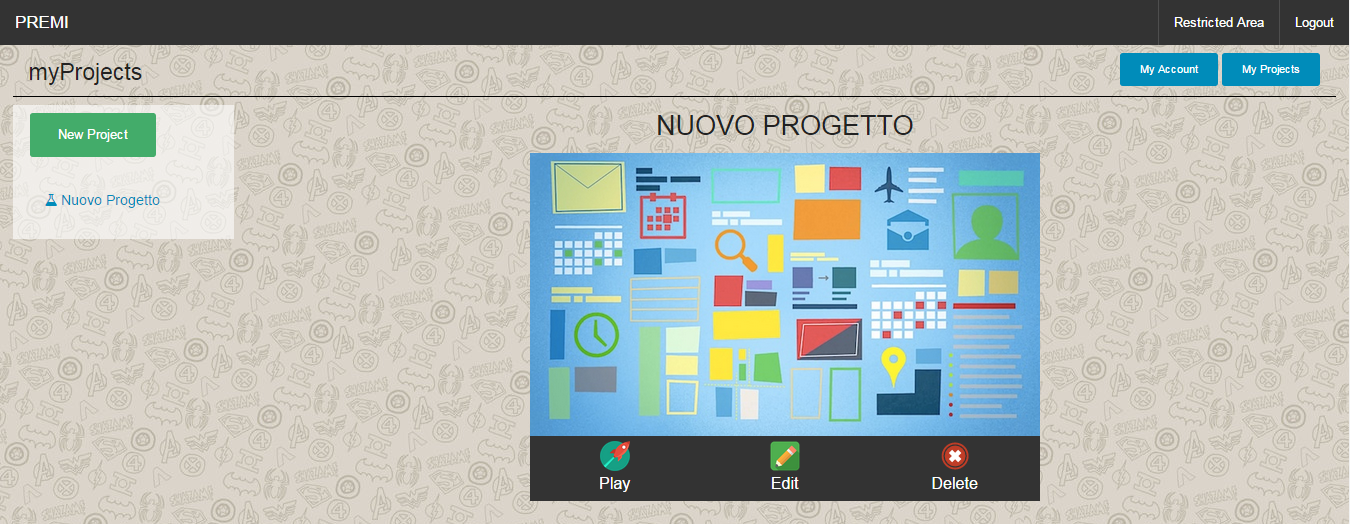
\includegraphics[scale=0.40] {img/presentazione.png}
	\caption{Creazione di una presentazione} 
\end{figure}